\documentclass[12pt]{article}

\title{\textbf{Image Analysis Coursework}}
\author{James Hughes\\ Word count: 2986}

\usepackage{amsfonts}
\usepackage{amsmath}
\usepackage{graphicx}
\usepackage{bm}
\usepackage{bbm}
\usepackage[a4paper, top=25mm, bottom=25mm]{geometry}
\usepackage{graphicx}
\usepackage[export]{adjustbox}

\begin{document}

\maketitle

\newpage

\tableofcontents

\newpage

\section{Image Segmentation}

\subsection{CT Image}

\begin{figure}[htp]
    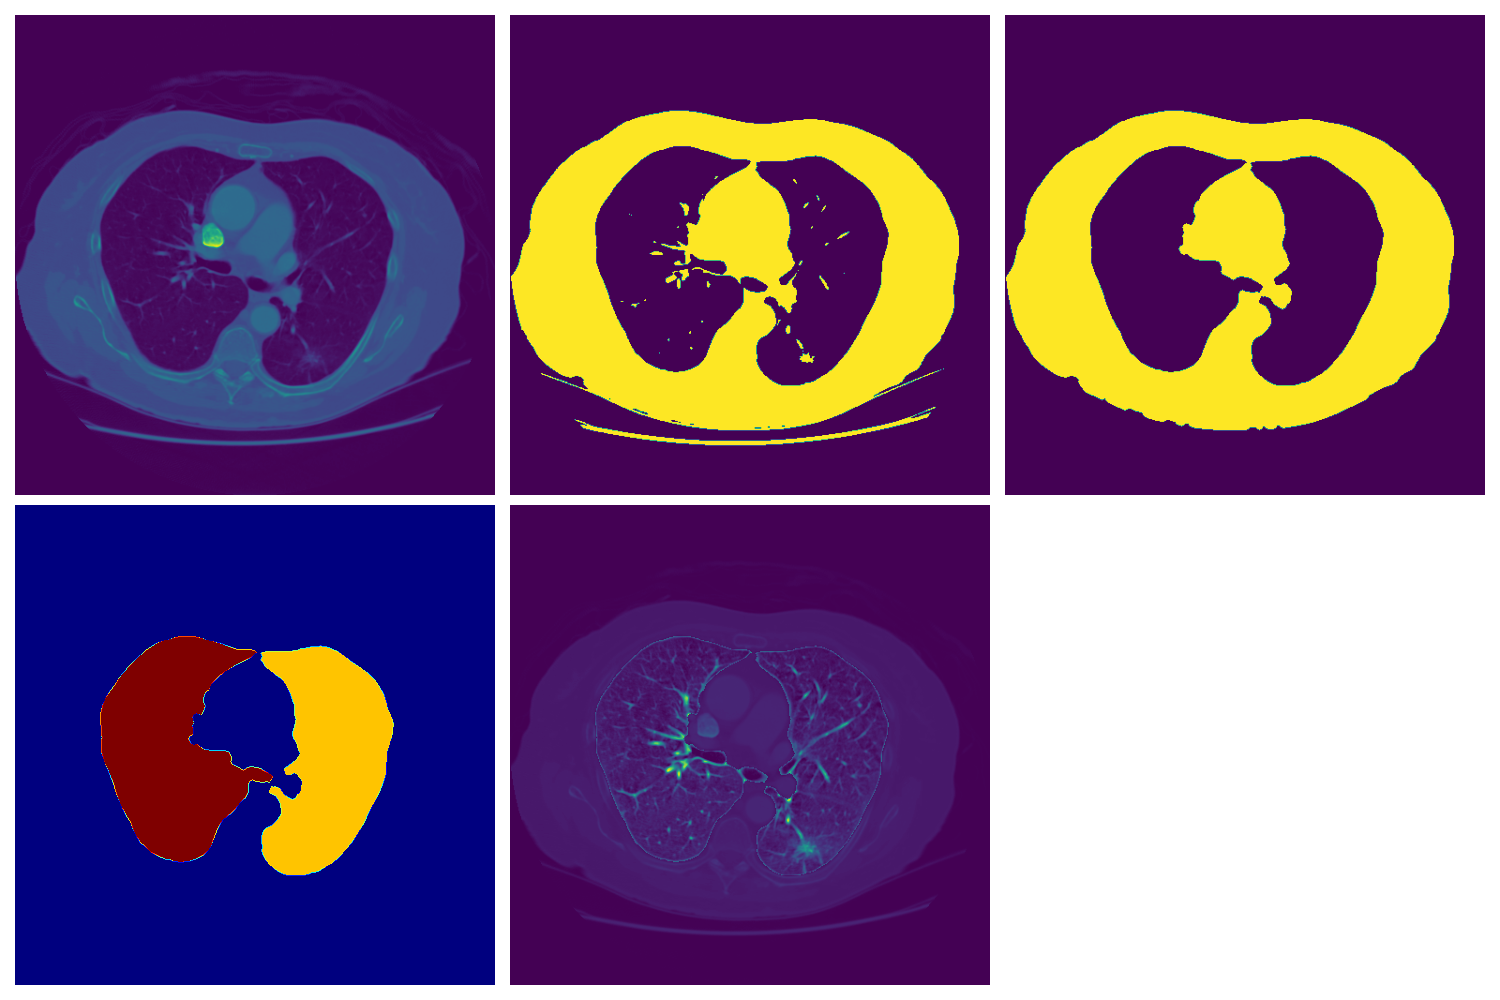
\includegraphics[scale=0.35, center]{figures/ct_segmentation.png}
    \caption{Steps of CT Segmentation. Top row: original image, segmentation mask, post-processing. Bottom row: individual lung masks, original image highlighted}
    \label{fig:ct}
\end{figure}

The CT scan image was segmented using Otsu's method for image segmentation.
This was an appropriate, simple method which is suited to the monochrome image.
This method easily segments the tissue and bone surrounding the lungs,
distinguishing this from the lugns themselves and the surrounding background.
The segmented image was then post-processed with `binary closing', a morphological operation,
as well as Scikit-Image's \texttt{morphology.remove\_small\_objects} method.
The four segmented regions of the image were then labelled, and the lungs chosen as the smallest masks by area.

\subsection{Flowers Image}

\begin{figure}[htp]
    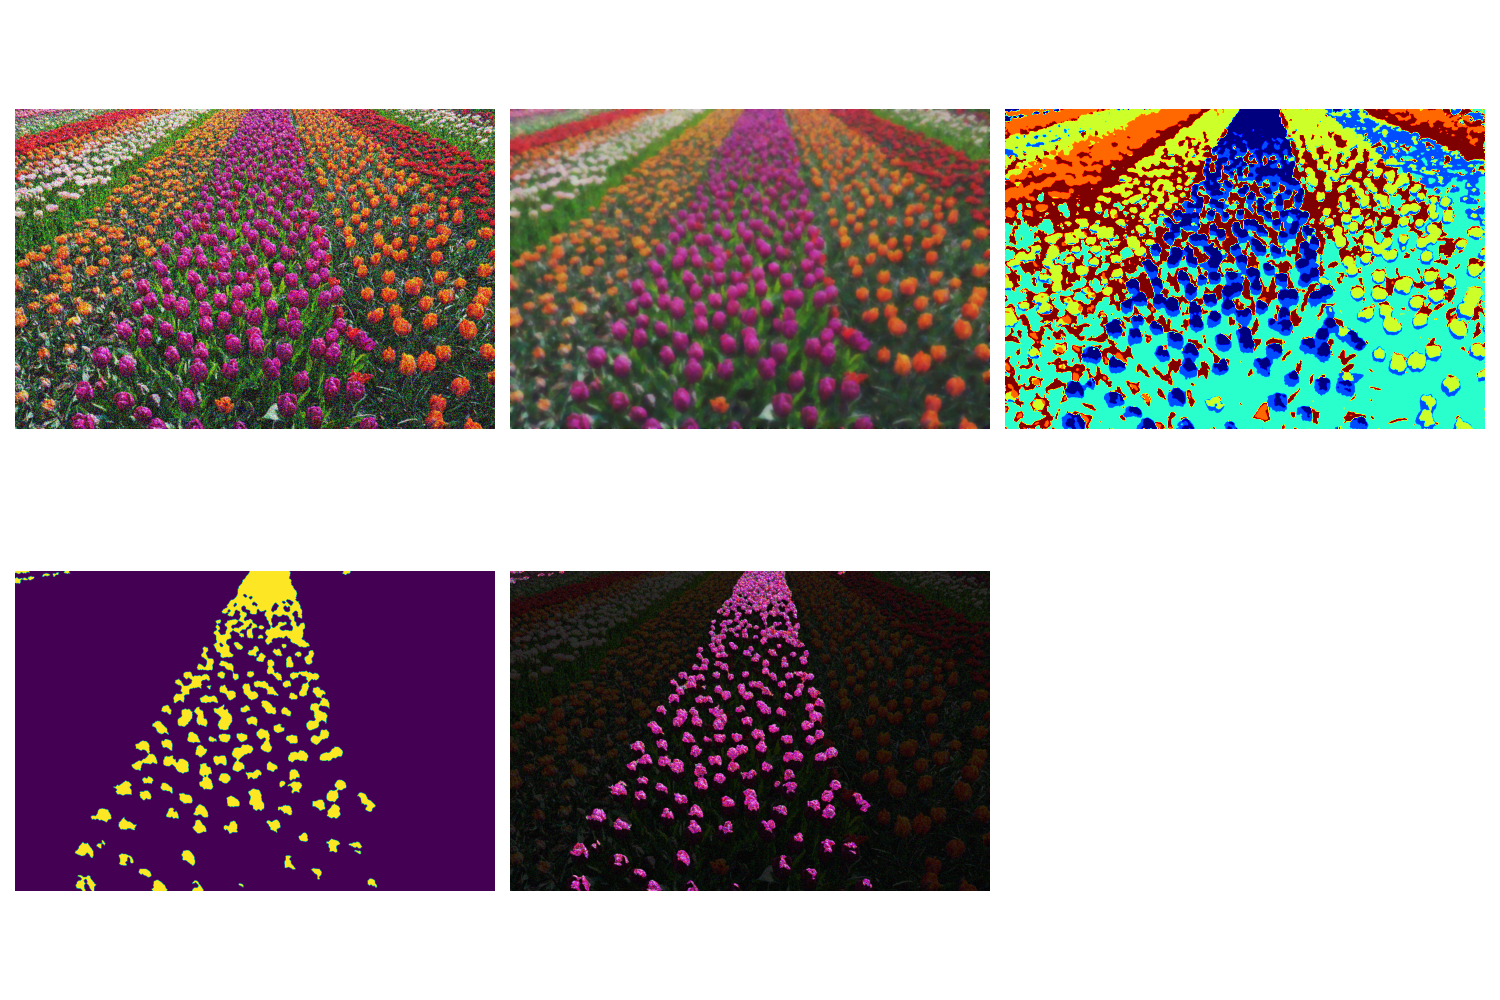
\includegraphics[scale=0.35, center]{figures/flowers_segmentation.png}
    \caption{Steps of Flowers Segmentation. Top row: original image, pre-processing, segmentation masks. Bottom row: post-processing, original image highlighted.}
    \label{fig:flowers}
\end{figure}

For the flowers image, a more sophisticated segmentation was required in order to handle the three colour channels of the pixels,
as well as to produce a more complex segmentation mask composed of lots of small disconnected regions.
Since the desired segmentation was to be based on the colours present in the image,
it was less important to incorporate local pixel information into the image,
therefore making clustering an appropriate strategy.
In particular, KMeans was chosen, since this method was simple to implement,
commonly used for image segmentation,
and enabled a fixed number of clusters to be specified.
In this case, six clusters was decided as a meaningful number,
corresponding roughly to two shades of green (grass) and four flower colours.
KMeans was implemented as a \texttt{class} in the \texttt{ml} module according to Lloyd's Algorithm \cite{lloyd},
using the kmeans++ \cite{kmeanspp} centroid initialisation method.

Based on this choice of algorithm, Total Variation (TV) denoising was used to pre-process the image.
This meant that in the pre-processed image, pixel values were coerced to be similar to those nearby.
This ensured that the clustering algorithm was more stable (since it artificially made the cluster structure of the data more pronounced),
and that the segmentation masks weren't too fine-grained.

The same morphological post-processing from the CT image was used again,
in order to remove segmentation masks that were smaller than the flower buds.

\subsection{Coins Image}

\begin{figure}[htp]
    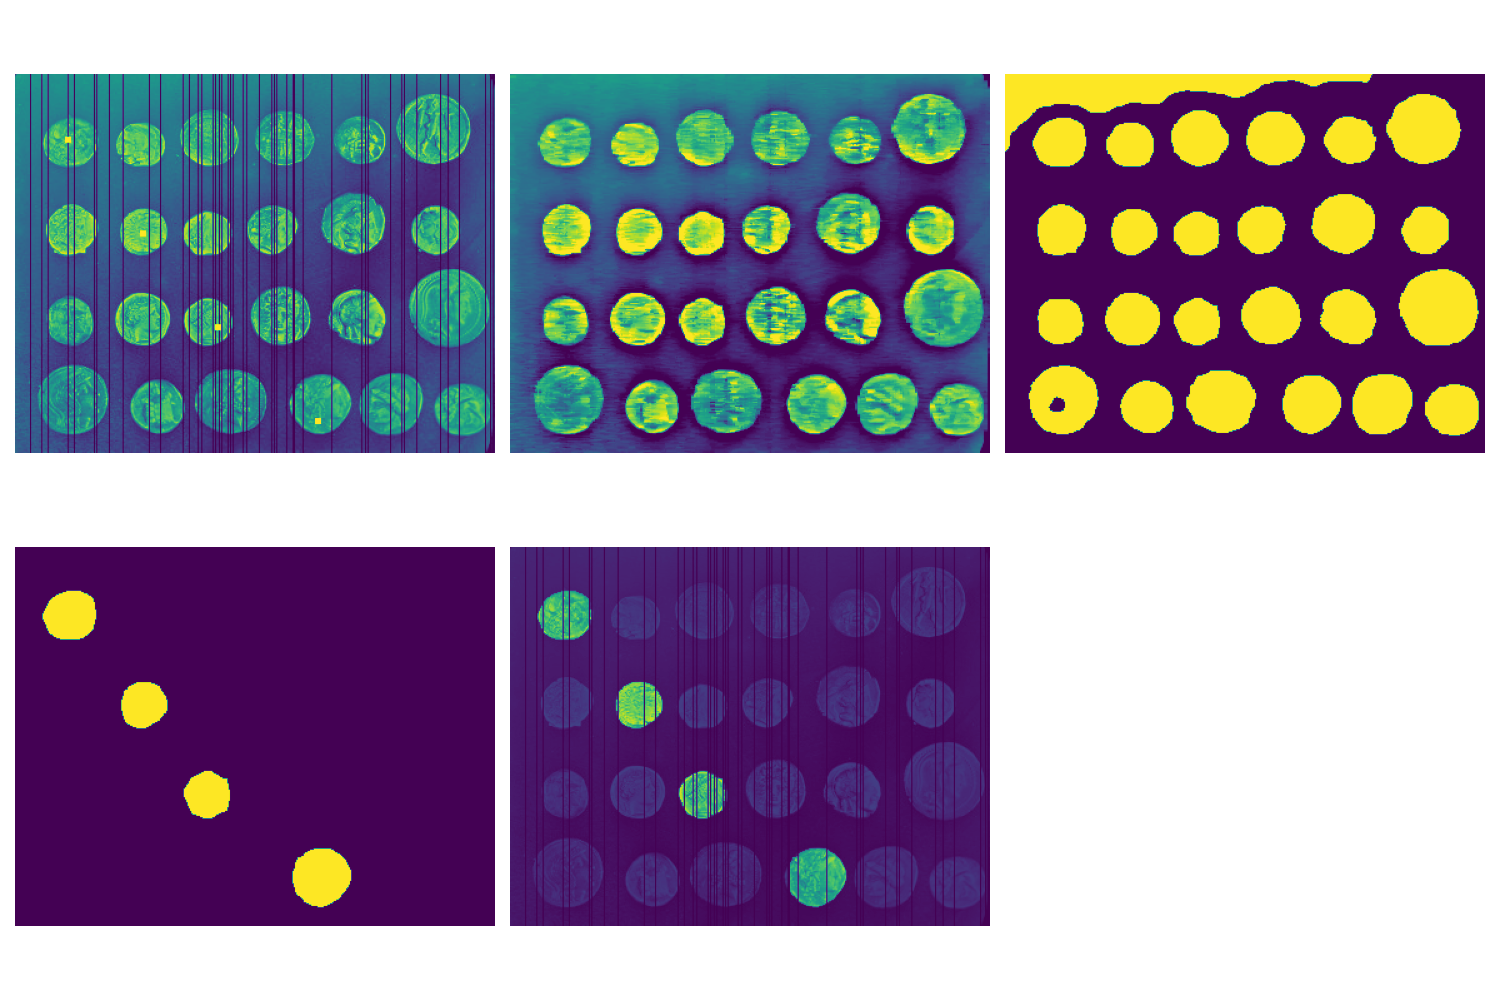
\includegraphics[scale=0.35, center]{figures/coins_segmentation.png}
    \caption{Steps of Coins Segmentation. Top row: original image (with coin markers in yellow), pre-processing, segmentation masks. Bottom row: selected masks, original image highlighted}
    \label{fig:coins}
\end{figure}

The image was corrupted with vertical columns of pixels that have been masked with zero values.
This was addressed by applying a local median filter.
The locality of this filter was set to each pixel plus its 6 closest horizontal neighbours.
This was wide enough to ensure that in most cases the majority of these 7 pixels were not corrupted,
even in regions where the image was affected more strongly.
An unsharp filter was then used to increase the pixel contrast at the edges of the coins.

To segment all of the coins, the Chan-Vese \cite{chanvese} segmentation algorithm was used.
This method relies on the iterative minimisation of an energy functional,
which describes the desired segmentation properties mathematically.
In particular, this technique models the segmentation mask as the set ${x\in\Omega:\phi(x)>0}$,
where $\Omega\subset\mathbb{R}^2$ is the space representing the image,
and $\phi:\Omega\rightarrow\mathbb{R}$ is a function which is optimised over the course of the computation.
The function $\phi$ is evolved iteratively to minimise the objective \cite{chanvese}

\begin{align*}
    F(\phi, c_1, c_2) = & \mu\int_{\Omega}\mathbbm{1}(\phi=0)|\nabla\phi|dxdy + \nu\int_{\Omega}\mathbbm{1}(\phi>0)dxdy \\
                    & + \lambda_1\int_{\Omega}|u_0-c_1|^2\mathbbm{1}(\phi>0)dxdy + \lambda_2\int_{\Omega}|u_0-c_2|^2\mathbbm{1}(\phi<0)dxdy \\
\end{align*}

where $\mu,\nu,\lambda_1,\lambda_2$ are all fixed hyperparameters, and $u_0:\Omega\rightarrow[0,1]$ is a function giving the image's pixel values.
The first two terms serve to regularise the segmentation,
by minimising the length of the segmentation boundary and the segmented area respectively (the area term is ignored in the code).
The second two terms seek to minimise the deviations of pixel values within, and outside, the segmented area from two distinct `representative values',
$c_1$ and $c_2$.
It is worth noting that for any $\phi$, these values minimise the energy when they are the average pixel values in the two corresponding areas of the image.

The algorithm highlighted the background of the image.
Thus to get masks of the coins, the segmentation values were permuted in $\lbrace0,1\rbrace$ and the segmentation was again post-processed with a morphological closing operation.
The masks were then labelled, and the correct labels were identified via `test pixels', which are seen marking the original image (top-left) in yellow in Figure \ref{fig:coins}.

\subsection{Discussion}

This part of the coursework highlighted to me some of the challenges of image segmentation.
In particular, it made me realise that it is important to match the method of segmentation,
and the pre-processing, to the segmentation task itself.
In the real-world, this can involve highly task-dependent choices---for instance the coins image task represents a scenario where the noise of the image is quite unusual,
and appropriate pre-processing must respond to the nature of the noise (as opposed to using some `generic' denoising method such as TV denoising).
In the same vein, it was interesting to revisit the lung segmentation task after using deep learning to perform a similar task in the medical imaging coursework.
The stark difference between the sophistication of the methods used there versus the simplicty and interpretability of the approach here is a helpful reminder to apply Occam's razor in data intensive science.
Additionally, this part showed me the sensitivity of the segmentation outcome with respect to the choice of pre-processing and parameters used.
This was particularly true in the KMeans clustering, where the number of clusters and the TV denoising parameters greatly affected the segmentation masks.
Implementing the KMeans algorithm explicitly, and researching the mathematics of the Chan-Vese algorithm also helped me to understand the mechanisms underlying these methods much better.

\section{Exploiting Sparsity in Signal Processing}

\subsection{Regression \& Outliers}

\begin{figure}[htp]
    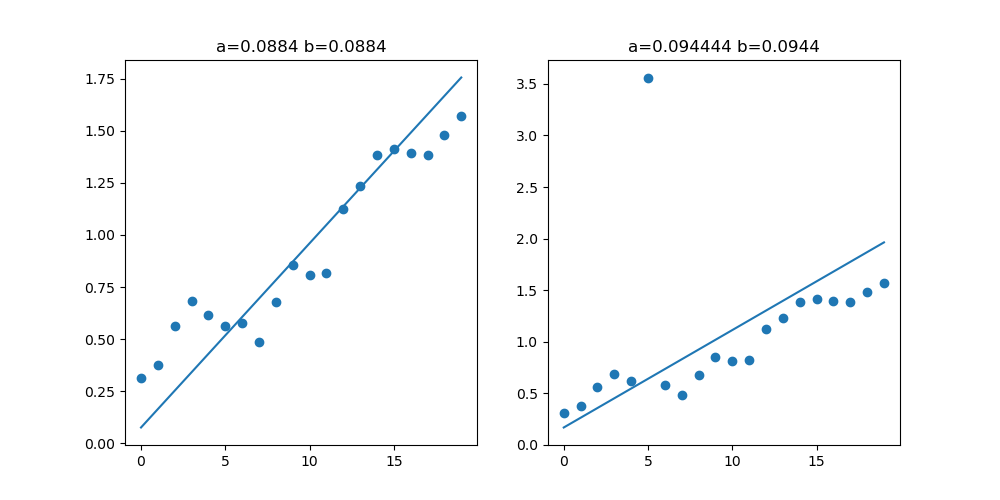
\includegraphics[scale=0.5, center]{figures/regression_l2.png}
    \caption{L2 Regression}
    \label{fig:regression_l2}
\end{figure}

For simple linear regression problems, the ordinary least squares approach for finding the coefficients is the most ubiquitous.
This is a well-posed optimisation problem that has an analytic solution, and also corresponds to a set of reasonable statistical assumptions in practical scenarios \cite{islp}.
This is due to the objective loss function being differentiable and strictly convex; indeed,
\[\text{minimise } \sum_{i=1}^{n}{(ax_i+b-y_i)^2} \quad \text{subject to } (a, b)\in\mathbb{R}^2\]
is therefore solved exactly by finding the unique argument for which the objectives gradient is zero,
\[a^*=\frac{\sum (x_i-\bar{x}) (y_i-\bar{y})}{\sum (x_i-\bar{x})^2},\quad b^*=\bar{y} - a^*\bar{x}\]

The original data and L2 regression models are plotted in Figure \ref{fig:regression_l2}.
Comparing the two models, we can see evidence that the least squares coefficients are quite sensitive to outliers.
In the second regression (where the data has the outlier) the coefficients change quite a lot,
so much that this model doesn't appear to fit the main body of data nearly as well as the first model,
even though only one outlier is present.

Using an L1 loss, under the so-called `Least Absolute Deviations' (LAD) model,
is designed to mitigate this sensitivity to outliers.
In both methods, the loss is the sum of some function of the residuals, the quantities $\hat{y_i} - y_i$ where $\hat{y_i}$ denotes the $i^{th}$ model prediction.
However, least squares regression uses the square of these residuals, so that the loss function, and therefore the solution, is much more sensitive to the largest residual values.
By replacing the squared residuals with the absolute residuals in LAD regression, all residuals contribute equally,
which means that the optimal LAD coefficients should be less sensitive to the presence of a few outliers.
On the other hand, the mathematics of the LAD regression framework is much more pathological.
The objective function is not differentiable, nor is it strictly convex, meaning that solutions are not guaranteed to be unique.
There is no analytic formula for any of the solutions.
Therefore the Subgradient Method was used to find the L1 coefficients.
This is similar to usual gradient descent, but extended to non-differentiable functions such as the L1 regression objective,
\[L(a,b) = \sum_{i=1}^{n}{|ax_i + b - y_i|}\]

We must replace the usual gradient term for the step direction with a non-unique `subgradient', a function $g:\mathbb{R}^2\rightarrow\mathbb{R}^2$ satisfying \cite{convex}
\[f(x')\geq f(x) + g(x)\cdot(x'-x) \quad \forall x, x' \in\mathbb{R}^2\]

\begin{figure}[htp]
    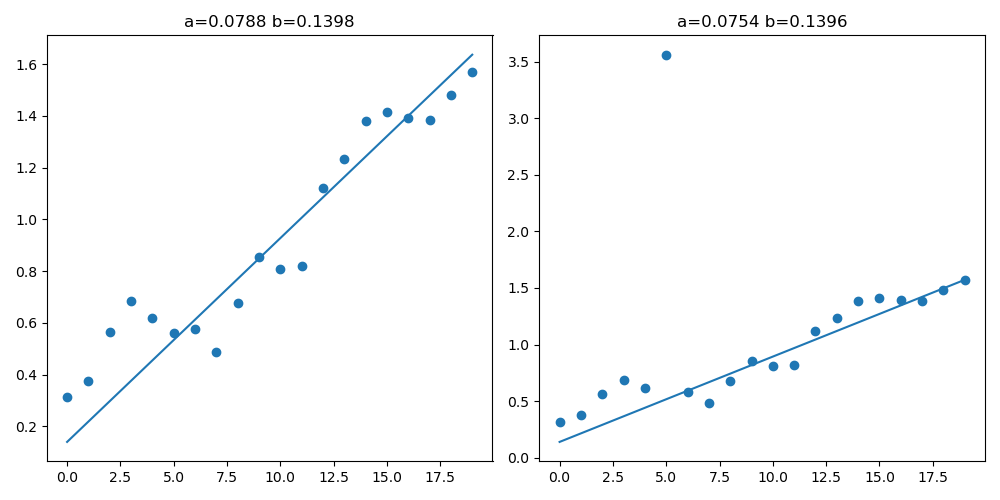
\includegraphics[scale=0.5, center]{figures/regression_l1.png}
    \caption{L1 Regression}
    \label{fig:regression_l1}
\end{figure}

All continuous convex functions such as the L1 objective permit a subgradient,
with non-uniqueness only at points of non-differentiability.
The subgradient chosen was based on a choice of subgradient for the function $z\rightarrow|z|$,
namely

\[
\text{sgn}(x) =
\begin{cases}
    1,   &\quad\text{if }x>0,\\
    -1,  &\quad\text{if }x<0,\\
    0,   &\quad\text{otherwise.}\\
\end{cases}
\]

which in turn gave the subgradient

\[x\mapsto(x^T\text{sgn}(ax+b-y), 1^T\text{sgn}(ax+b-y))\]

where $\text{sgn}$ is applied elementwise.
The results of the Subgradient Method regression are shown in Figure \ref{fig:regression_l1}.
We see that this method is much more robust against outliers, with similar coefficients found in both cases.
In addition, the coefficients found for the non-outlier case are fairly similar to the least squares coefficients.
The downsides of this method are that the coefficients are somewhat sensitive to the choice of learning rate and initial coefficient.

\subsection{Undersampling} \label{section:undersampling}

In this part we reconstruct a sparse signal from two different samples of its transformation into k-space.
We create a vector with only 10\% non-zero entries and then add a small amount of Gaussian noise to simulate a sparse signal.
We then Fourier transform this and take two 4-fold undersampling strategies:
\begin{itemize}
    \item equidistant sampling; where every fourth entry in k-space is sampled (though the offset is randomly chosen), and,
    \item random sampling; where exactly one quarter of the entries are sampled, each entry having equal selection probability.
\end{itemize}
In both cases, the non-sampled entries in k-space are masked with zeros.

\begin{figure}[htp]
    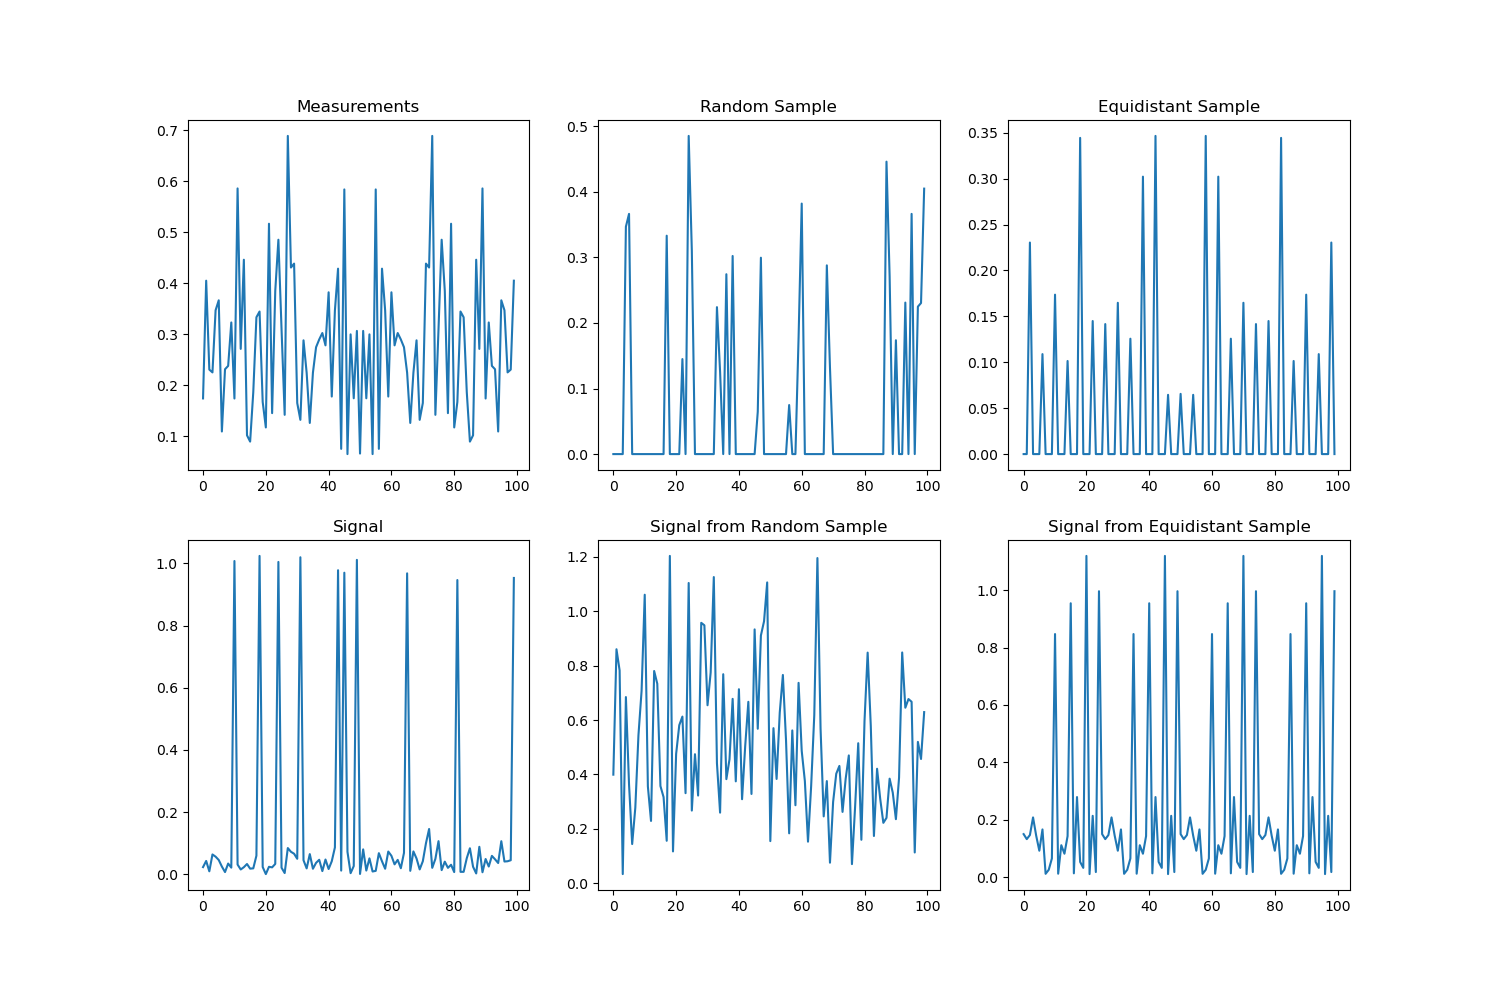
\includegraphics[scale=0.36, center]{figures/signal.png}
    \caption{Signals and measurements (absolute values)}
    \label{fig:signal}
\end{figure}

The samples simulate measurements ($y$) taken in a real-life scenario, which are some function of the true underlying signal ($x$),
in this case the signal's Fourier transform.
In both cases the samples were used to reconstruct the signal via Iterative Soft Thresholding,
which in this case involved repeating the following steps
\begin{itemize}
    \item transforming to the signal domain (inverse Fourier transform),
    \item soft-thresholding the approximate signal,
    \item transforming back to the measurement domain (Fourier transform), and,
    \item enforcing data consistency with the original measurements.
\end{itemize}

In Figure \ref{fig:signal_reconstruct} we see the results of this reconstruction using 100 iterations and $\lambda=0.02$ for the soft-thresholding.
Importantly, the algorithm only had an effect on the signal that was inferred from the random sample of measurements.
In this case, the algorithm improved the accuracy of the signal reconstruction,
as shown by the L2 distance of the reconstructed measurements compared to the true measurements decreasing over time.

\begin{figure}[htp]
    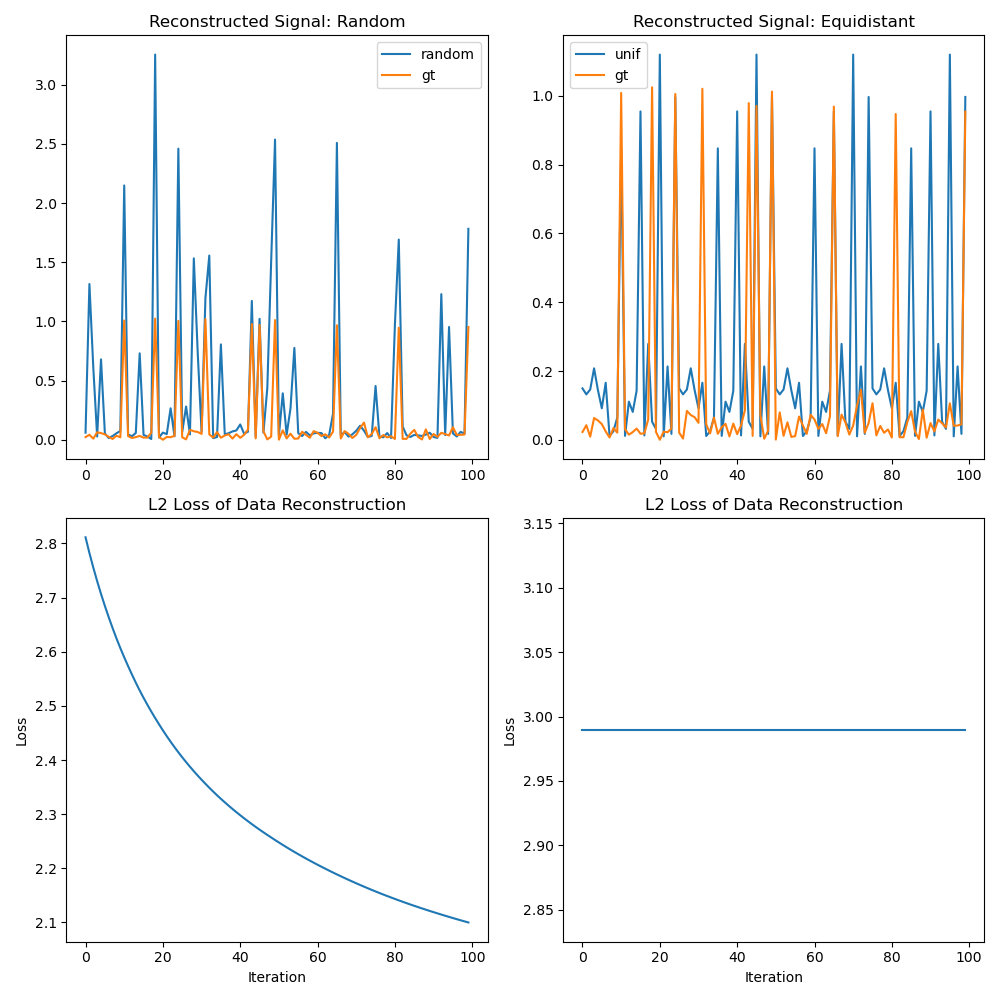
\includegraphics[scale=0.5, center]{figures/signal_reconstruct.png}
    \caption{Iterative Soft Thresholding Reconstructions}
    \label{fig:signal_reconstruct}
\end{figure}

This case study serves as a demonstration of the power of Compressed Sensing,
when done correctly.
Compressed Sensing emerged in the signal processing literature in the mid 2000s,
offering a radically efficient way of acquiring signals using far fewer measurements than suggested by classical results in the field \cite{candes2005stable}.
The well-established Nyquist-Shannon sampling theorem suggests that the sampling rate should be more than twice the greatest frequency present in the true data,
as this ensures perfect signal reconstruction according to the result \cite{shannon}.
However, this sampling rate is notably framed as a sufficient, rather than necessary condition in the theorem,
and Compressed Sensing develops a framework in which under certain assumptions,
an excellent signal reconstruction can occur with a much more economical sampling scheme.
In particular, we must assume \cite{cs}:
\begin{enumerate}
    \item incoherence; this is achieved in general by a `random' subsampling scheme, and,
    \item sparsity; the measurements must have a sparse representation in some transformed domain, such as Fourier or wavelet decomposition.
\end{enumerate}

By undersampling by a factor of 4 we generate a highly underdetermined inverse problem,
namely that infintely many signals $x$ can be mapped to the measurements $y$ by the Fourier transform and 4-fold undersampling.
Heuristically, the assumption of sparsity of $x$ `narrows down' this pool of candidate signals,
leading to a more accurate reconstruction of the signal in the random sampling scheme.
The equidistant sampling scheme violates the first assumption of incoherence,
leading to a reconstruction which cannot be improved.
This scheme leads to the `aliasing' effect that the Nyquist-Shannon sampling theorem was designed to mitigate against.
Namely, by undersampling in this way, high frequency components in the data are confounded with low frequency components,
consituting an irreversible loss of information \cite{cs}.

\subsection{Wavelet Decomposition}

\begin{figure}[htp]
    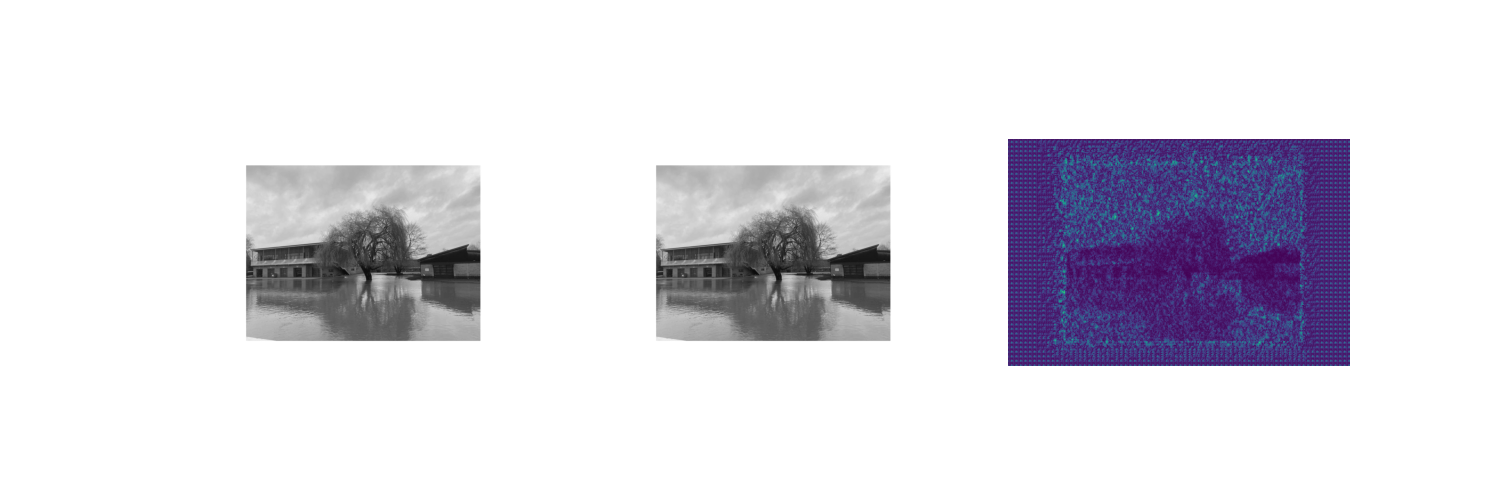
\includegraphics[scale=0.45, center]{figures/river_img.png}
    \caption{River Image and Reconstruction from Wavelet Decomposition}
    \label{fig:river_img}
\end{figure}

\begin{figure}[htp]
    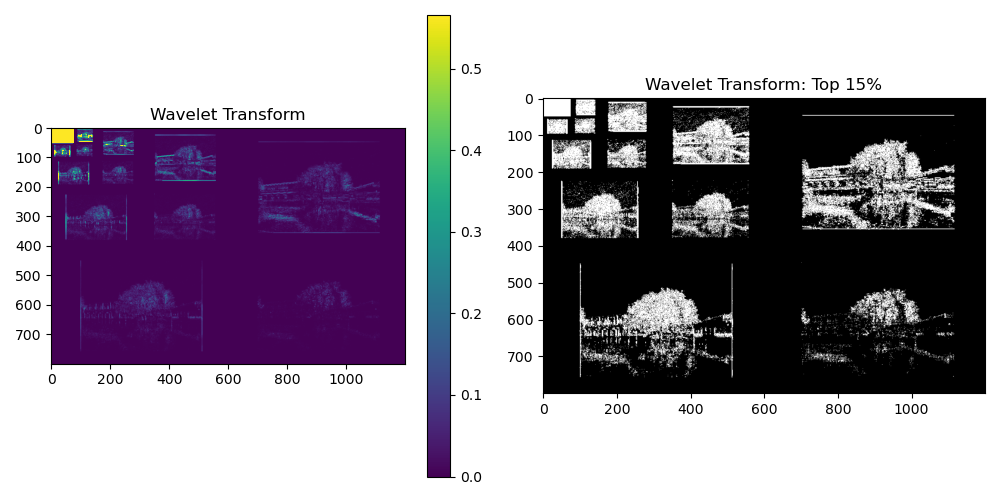
\includegraphics[scale=0.5, center]{figures/wavelet_transform.png}
    \caption{River Image and Reconstruction from Wavelet Decomposition}
    \label{fig:wavelet_transform}
\end{figure}

In this part, we explore the relevance of sparsity to image processing.
Figure \ref{fig:river_img} (left) shows an image which was passed through a Daubechies wavelet transform.
The two other images show the effects of reconstructing this image by directly applying the inverse wavelet transform.
The reconstruction is almost identical to the original, achieving a Structural Similarity Index which is perfect to two decimal places.
Crucially, the right-most image in Figure \ref{fig:river_img} shows that where there are pixel value errors,
they are greatest in the main central part of the image (where this plot is brighter on average).
The errors are generally smaller in the empty space around the image, although there is an unusual periodic pattern of errors here.

Figure \ref{fig:wavelet_transform} shows the wavelet transform of the river image.
On the left we see the original coefficients\footnote{clipped in the 0.5-99.5\% range to improve visibility},
while the right hand side indicates which of these lie in the top 15\% of coefficients.
We see that even removing 85\% of the expressive range of the coefficients in the wavelet domain,
the representation still encodes meaningful features relating to the image - this is a sparse representation of the image.

\begin{figure}[htp]
    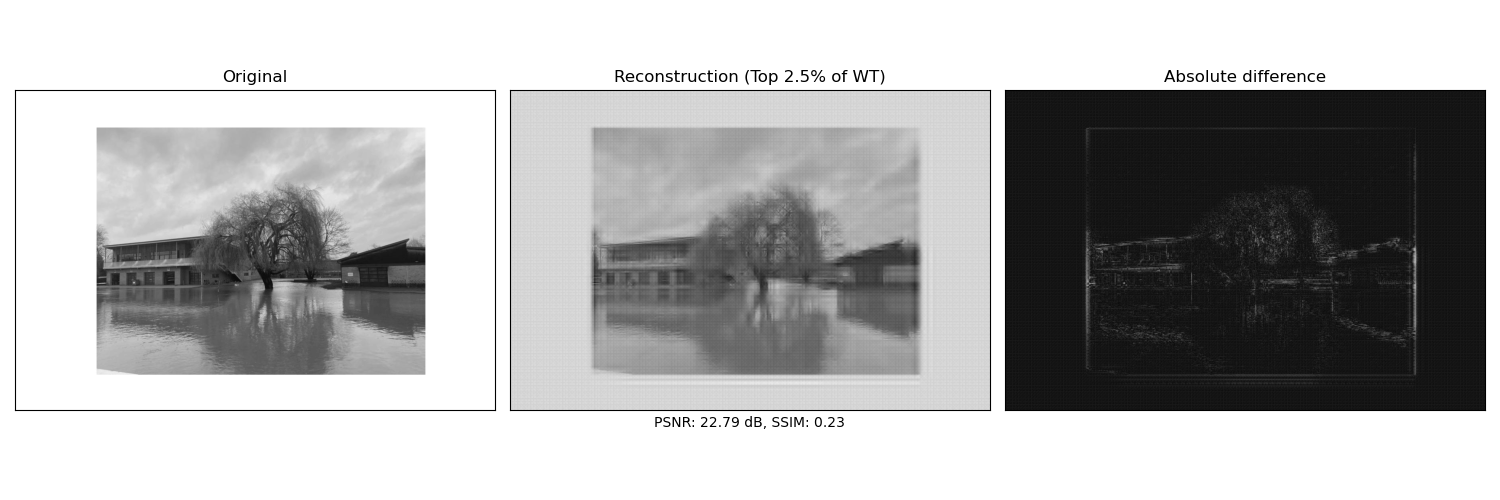
\includegraphics[scale=0.45, center]{figures/river_img_compressed_0.025.png}
    \caption{Compression from removing 97.5\% of wavelet information}
    \label{fig:river_3pct}
\end{figure}

\begin{figure}[htp]
    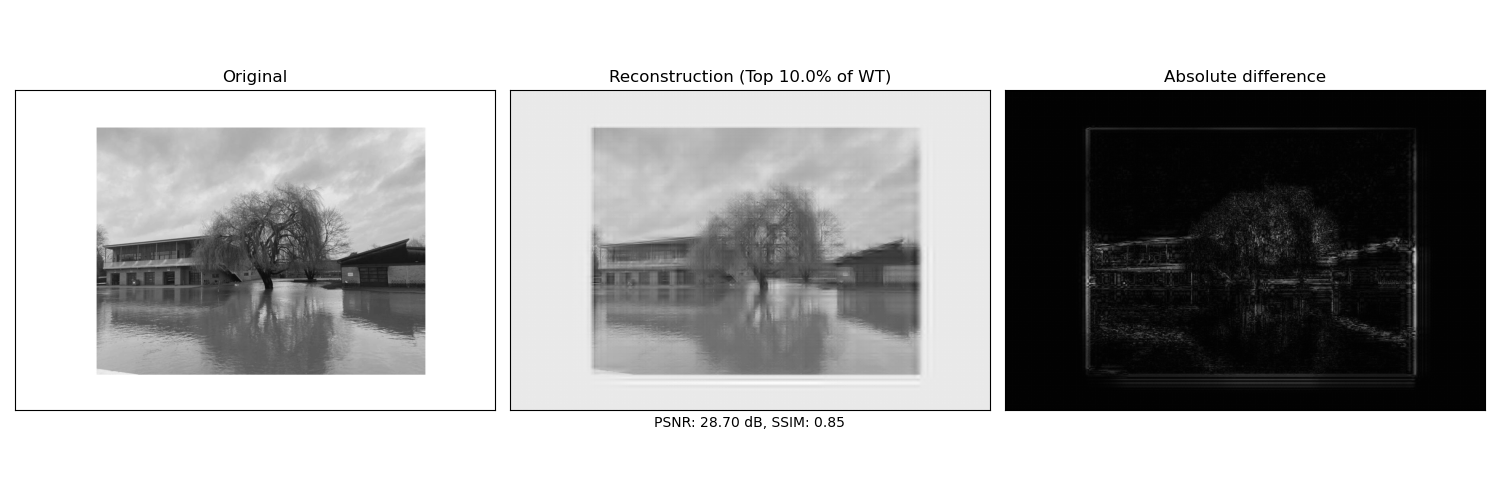
\includegraphics[scale=0.45, center]{figures/river_img_compressed_0.100.png}
    \caption{Compression from removing 90.0\% of wavelet information}
    \label{fig:river_10pct}
\end{figure}

\begin{figure}[htp]
    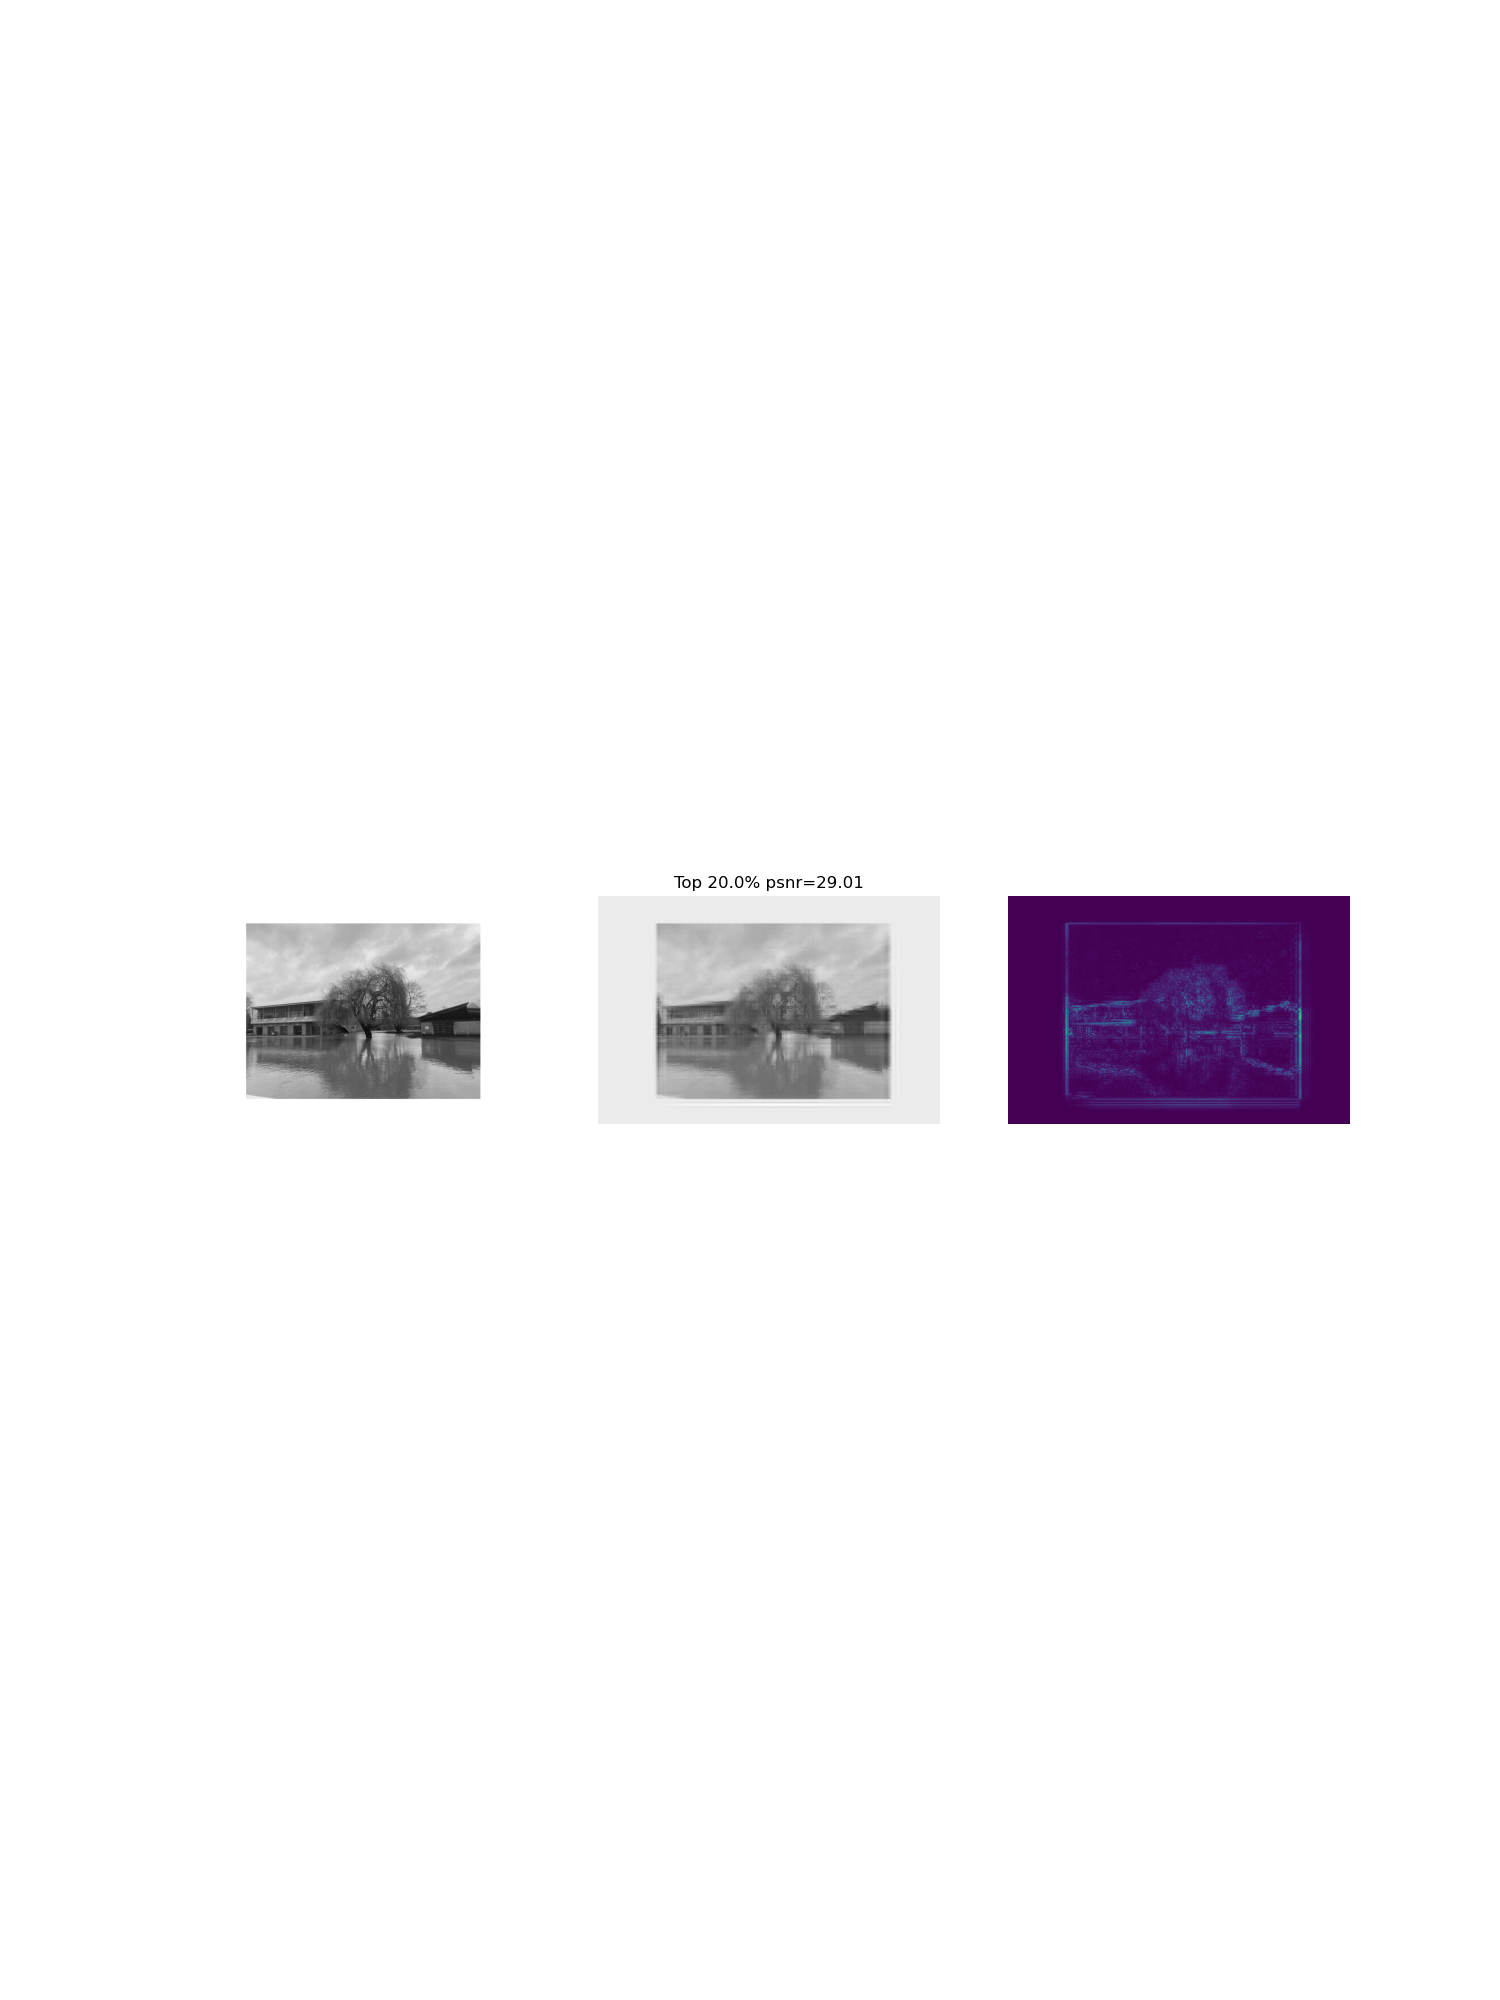
\includegraphics[scale=0.45, center]{figures/river_img_compressed_0.200.png}
    \caption{Compression from removing 80.0\% of wavelet information}
    \label{fig:river_20pct}
\end{figure}

As a result, zero-filling coefficients whose absolute value is below this threshold and then performing the inverse transform produces an image which is highly faithful to the original,
but also requires dramatically less digital storage space, if we properly exploit the sparse representation to save the image.
This is the essence of image compression techniques.
The results of this compression can be seen at different threshold values in Figures \ref{fig:river_3pct}, \ref{fig:river_10pct}, and \ref{fig:river_20pct},
with more examples in the \texttt{/report/figures} folder.

Strikingly, we see that even the extreme compression in Figure \ref{fig:river_3pct} is fairly faithful visually to the original.
However, the more intense the compression process, the further the image is degraded.
As we remove increasing amounts of wavelet-domain data, the difference image changes from a `blur' in the central region,
to showing the worst errors concentrated around the high spatial frequency features of the images (details like edges and corners).
In Figure \ref{fig:river_3pct} this is most obvious for the leaves of the tree and its shadow,
which loses some fidelity in the compressed image and becomes more blurred.

\subsection{Discussion}

The common thread through these three different tasks is the exploitation of the concept of sparsity to achieve a somewhat similar goal in all cases.
Namely, we were given some data or measurements and wanted to find an efficient, lower-dimensional representation of it.
The approach was to make a prior assumption of sparsity in some related, transformed domain.
In the regression problem, the lower dimensional representation was in two dimensions (the regression coefficients),
with the transformation of the data
\[(x_i,y_i)\mapsto |ax_i+b-y_i|\]
leading to sparsity. In the other two problems, the data was transformed via Fourier or wavelet transforms in order to exploit sparsity.
In this way, this part enabled me to see the links between areas of signal processing which appear to be quite different on the surface.

\section{Algorithms for Solving Inverse Problems}
\subsection{Convergence of Gradient Descent}

When applied to a convex, $L$-smooth objective function $f$ with learning rate $\eta=\frac{1}{L}$,
gradient descent is guaranteed to converge with accuracy

\[f(\bm{x}_K) - f(\bm{x}^*) \leq \frac{L||\bm{x}_0-\bm{x}^*||_2^2}{2K}\]

where $K\in\mathbb{N}$ is the iteration number \cite{garrigos2024handbook}.

It is important to note that this is an estimate that gives the accuracy as $\mathcal{O}(\frac{1}{K})$.
We can use it to compute the estimate the number of steps to required to achieve accuracy $\epsilon=0.01$,
but this will be an upper bound.
Nonetheless, we can set the left-hand side to $\epsilon$ and rearrange to give:

\[K \leq \frac{L||\bm{x}_0-\bm{x}^*||_2^2}{2\epsilon}\]

We can prove that the given function $f:\mathbb{R}^2\rightarrow\mathbb{R}$ defined

\[f(x_1,x_2) = \frac{x_1^2}{2} + x_2^2\]

is $L$-smooth with $L=2$ by observing

\[\nabla f(x_1, x_2) = (x_1, 2x_2),\]

and,

\begin{align*}
    ||\nabla f(\bm{x}) - \nabla f(\bm{x}')||_2^2 & = (x_1-x_1')^2 + (2x_1-2x_1')^2 \\
                                            & = (x_1-x_1')^2 + 4(x_1-x_1')^2 \\
                                            & \leq 4(x_1-x_1')^2 + 4(x_1-x_1')^2 \\
                                            & = 4||f(\bm{x}) - f(\bm{x}')||_2^2, \\
\end{align*}

which proves that,

\[
    ||\nabla f(\bm{x}) - \nabla f(\bm{x}')||_2 \leq 2||f(\bm{x}) - f(\bm{x}')||_2.
\]

Hence we substitute $\epsilon=0.01$, $x^*=(0,0)$, $x_0=(1,1)$, $L=2$ into the estimate for the number of steps required.
We obtain $K=200$.

In practice, the number is indeed much smaller; it was found to require just 3 iterations with the prescribed step size $\eta=0.5$.
The left image in Figure \ref{fig:gradient_descent} shows the trajectory of this iterative solution.
On the right, we see a very fast convergence of the value of the function $f$ towards its true global minimum zero.

\begin{figure}[htp]
    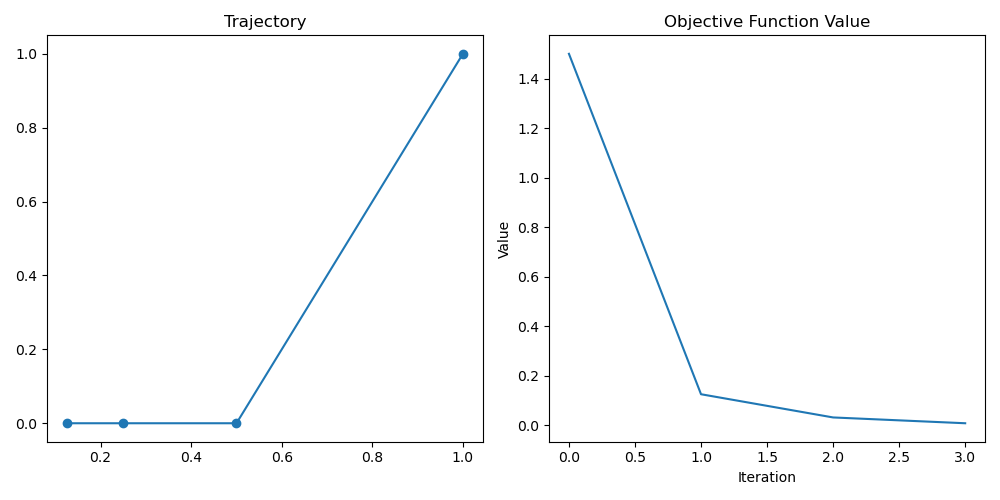
\includegraphics[scale=0.5, center]{figures/gradient_descent.png}
    \caption{Results of Gradient Descent Algorithm}
    \label{fig:gradient_descent}
\end{figure}

\subsection{Learned Gradient Descent}

In this section, we compare the results of solving some linear inverse problem using a classical direct approach,
a model-based minimisation, and a data-driven method.
The task is to reconstruct a medical image from a sinogram,
which is the set of measurements taken by a computed tomography scan.
The forward operator in this case is the linear `Radon transform'.

The simplest way to achieve a reasonable reconstruction is to use the filtered backprojection (FBP) algorithm.
The FBP applies a 1D `ramp' filter to measurements in the sinogram,
thereby upweighting its high-frequency components,
and then applies the adjoint operator to approximate the inverse of the forward projection,
yielding an image.

\begin{figure}[htp]
    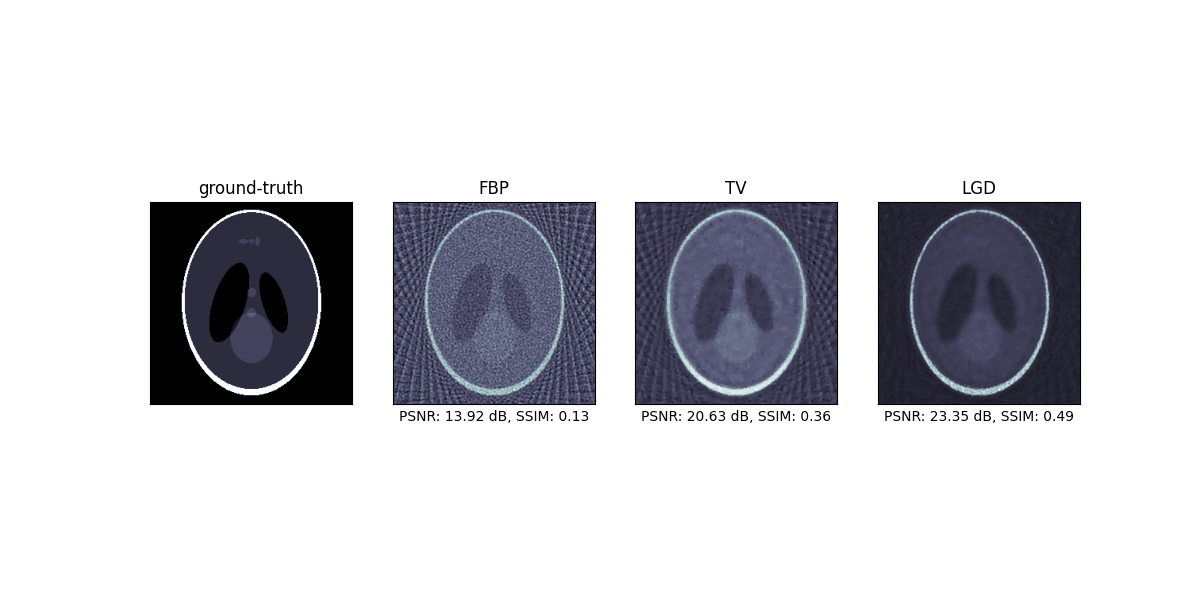
\includegraphics[scale=0.65, center]{figures/lgd.png}
    \caption{Reconstruction of CT Scan Using Learned Gradient Descent Compared to Filtered Backprojection and Alternative Direction Method of Multipliers}
    \label{fig:lgd}
\end{figure}

Secondly the Alternative Direction Method of Multipliers (ADMM) algorithm was used.
This is an iterative, model-based approach that minimises an objective which is composed of an L2 fidelity term, plus an L1 regularisation term.
We already saw this problem solved earlier in Section \ref{section:undersampling}.
However, in the earlier signal processing problem, the underlying signal (the goal of reconstruction) was the sparse representation,
and therefore the subject of the L1 regularisation, permitting a simple Iterative Soft-Thresholding strategy.
In this case, it is instead a linear transform of the signal (the image) -- namely its total variation -- which is regularised,
so that a more sophisticated solution---ADMM---is required.

Both of the previous strategies have strong pre-suppositions of the imaging physics embedded into them.
In the ADMM approach for instance, we can draw an equivalence between the use of total variation regularisation,
and employing a prior distribution on $x$ which asserts that the image is likely to belong to a manifold of low-noise images with respect to the L1 TV score.
Learned Gradient Descent (LGD) is, by contrast, a data-driven approach which, heuristically, `learns' the regularisation based on its exposure to samples of ground truth images.
This means that this embedded bias of the model can be fine-tuned more closely to the specific class of images that are relevant.
On the other hand, it makes the model much less transparent and prohibits certain theoretical guarantees that are present with the earlier approaches.

Figure \ref{fig:lgd} shows a comparison of all three image reconstructions.
We can see that the LGD performs the best both quantitatively,
and in terms of mitigating the reconstruction artifacts that affect the other two approaches.
However, this is quite an unfair comparison due to the model being trained, and then evaluated, on the same single image.

\subsection{Discussion}

The first task in this part is an important reminder that empirical results often deviate from what one might expect based on theory.
In this task, we see a guarantee of convergence within a certain number of iterations being a large overestimate,
but it is worth noting that in the context of the applications of gradient descent,
the objective function here has some very helpful properties in terms of convergence analysis.
In practice, especially in deep learning, gradient descent (and extensions of it) is used to optimise high-dimensional non-convex loss functions that are prone to many local minima as well as saddle points,
leading to even more unusual behaviour of the method.
The example using LGD showed how powerful new data-driven strategies can be in image processing,
as well as the computational challenges in developing them.

\bibliographystyle{IEEEtran}
\bibliography{Biblio}

\appendix

\section{Statement on the use of auto-generation tools}

Auto-generation tools, such as GitHub Copilot or Microsoft Copilot, were not used at any stage during the development of the code within the repository of this project.
Similarly, none of the content of this report was produced -- or proofread -- by modern Large Language Models such as ChatGPT at any point.

\end{document}
